\documentclass{article}

\usepackage{arxiv}
\usepackage[utf8]{inputenc}
\usepackage[T1]{fontenc}
\usepackage{graphicx}
\usepackage{booktabs}
\usepackage{amsmath}
\usepackage{amssymb}
\usepackage{multirow}
\usepackage[numbers]{natbib}
\usepackage{microtype}
\usepackage{xcolor}
\usepackage{newtxtext,newtxmath}
\usepackage{caption}
\usepackage[hidelinks]{hyperref}

\captionsetup{font=small,labelfont=bf,width=.94\linewidth}
\setlength{\textfloatsep}{10pt plus 2pt minus 2pt}
\setlength{\floatsep}{8pt plus 2pt minus 2pt}
\setlength{\intextsep}{8pt plus 2pt minus 2pt}

\definecolor{deepteal}{HTML}{0B6E69}
\definecolor{inkblue}{HTML}{2F5D8A}
\definecolor{warmred}{HTML}{B64B3C}
\definecolor{softgray}{HTML}{5F6872}

\newcommand{\sysname}{\textsc{maxsim}}
\newcommand{\ndcg}{NDCG@10}
\newcommand{\recall}{Recall@10}
\newcommand{\fp}{\textsc{fp}}

\title{\textsc{maxsim}: Model-Aware Compression for Multi-Vector Retrieval}

\author{Arya Manjaramkar\\
\href{https://github.com/Aryagm/maxsim}{github.com/Aryagm/maxsim}}

\date{July 2026}

\renewcommand{\shorttitle}{\textsc{maxsim}}
\renewcommand{\headeright}{Preprint}
\renewcommand{\undertitle}{Preprint}

\begin{document}
\maketitle

\begin{abstract}
Multi-vector retrieval improves accuracy by retaining a vector for every query
and document token, but the resulting indexes are expensive to store and
score. We present \sysname{}, a compression and CUDA runtime for
fixed-dimensional dot-product late interaction. Its representations span
$3.76\times$--$95.9\times$ compression relative to fp32, and its shared
reducers implement MaxSim, weighted MaxSim, TopK2, TopK4, and SmoothSim.

The central empirical result is that aggressive compression is
\emph{model-dependent}. We evaluate four text and visual encoder families
across 20 encoder--dataset combinations. Per-token int8 is the conservative
control: it remains within 0.0063 \ndcg{} of dense in every evaluated cell.
Per-token int4 is nearly lossless for Jina-ColBERT-v2 and the visual encoders,
but loses 0.065 mean \ndcg{} on GTE-ModernColBERT. Binary and pooled-binary
formats retain roughly 98\% of dense quality on the visual suites at
$32\times$ and approximately $96\times$ compression, yet their losses are
substantially larger for GTE. Thus none of the evaluated aggressive codecs is
a defensible universal default across the tested encoders; the default must
be a small, model-aware calibration procedure over a portfolio.

We validate the systems consequences on 10,171 visual documents and 57,638
text documents. On the visual corpus, binary and pool3 reduce single-query
full-scan latency from 85.7\,ms to 3.32\,ms and 2.17\,ms while using 16.0 and
47.9 times less storage than fp16. Across 24 nested-scale runs, these speedups
remain consistent as the corpus grows. The five reducers match PyTorch within
$2.44{\times}10^{-4}$, and candidate-only scoring is $4.5\times$--$5.7\times$
faster than full scoring at 4,096 documents. We release the library, exact
result artifacts, checksums, and deterministic paper-generation code.
\end{abstract}

\section{Introduction}

Late-interaction retrieval~\citep{khattab2020colbert} represents a query and
document as sets of vectors and aggregates token-level similarities only at
search time. This design supports strong text retrieval and, through
ColPali-style encoders~\citep{faysse2025colpali}, direct retrieval over
document images. It also changes the deployment bottleneck. A single
document may contain hundreds of token or patch vectors, so even a modest
corpus can require gigabytes of accelerator memory and a large dot-product
reduction for every query.

Compression is the natural response, but ``which compression method should be
the default?'' remains operationally unresolved across encoder families.
Binary signs, scalar quantization, token pooling, and residual codes make
different assumptions about embedding geometry. A method that is nearly free
for one encoder may erase useful structure for another. Evaluations on one
model or one corpus cannot reveal that failure mode.

This paper studies compression as a \emph{portfolio} rather than a single
codec. \sysname{} stores the same multi-vector index in several formats,
scores the stored similarities with parity-tested CUDA kernels, and exposes a
common reducer interface. We then ask three practical questions:

\begin{enumerate}
\item Which formats preserve retrieval quality across text and visual
encoders?
\item How do the quality, storage, and latency trade-offs behave as the
benchmark corpus grows?
\item Does the runtime extend beyond MaxSim without duplicating a custom
kernel for every late-interaction reducer?
\end{enumerate}

The answers are useful precisely because they are not uniform. Per-token int8
is consistently near dense, but its $3.88\times$ compression versus fp32 is
modest. Per-token int4 provides a stronger $7.53\times$ point and is
near-lossless for Jina and both visual families, but not for GTE.
Binary and pool3 provide the largest latency and storage gains on visual
documents, while GTE needs a higher-fidelity representation. The result is a
simple deployment rule: use a conservative control, measure a handful of
aggressive formats on a held-out query set, and choose the smallest format
that meets the application's quality budget.

Our contributions are:

\begin{enumerate}
\item \textbf{A unified compression runtime.} The released representations
cover $3.76\times$--$95.9\times$ compression versus fp32. A shared CUDA
reducer supports five dot-product late-interaction scorers over binary and
int4 indexes, for both full-corpus and candidate-only scoring.
\item \textbf{A controlled cross-model map.} Four encoder families and 20
encoder--dataset evaluations show that compression behavior is
encoder-dependent, not determined by modality alone. Per-token int8 provides
a near-lossless control; the best aggressive tier must be calibrated.
\item \textbf{Systems and scale evidence.} Two end-to-end corpora, 24
nested-scale runs, matched FastPLAID baselines, and raw latency distributions
quantify quality, storage, throughput, and index lifecycle costs on one
RTX~4090.
\end{enumerate}

\section{Background and System}

\subsection{A common late-interaction interface}

Let a query contain vectors $q_1,\ldots,q_m$ and document $d$ contain vectors
$x_1,\ldots,x_n$. We write a family of dot-product late-interaction scorers as
\begin{equation}
S(q,d)=\sum_{i=1}^{m} w_i\,
\rho\!\left(\left\{\langle q_i,x_j\rangle\right\}_{j=1}^{n}\right),
\label{eq:general}
\end{equation}
where $\rho$ is a reducer over document tokens. MaxSim uses a maximum and
$w_i=1$. Weighted MaxSim changes $w_i$; TopK2 and TopK4 aggregate the largest
two or four similarities; SmoothSim replaces the hard maximum with a
temperature-controlled smooth reduction.

Compression changes how each dot product is reconstructed, but not the
reduction structure. This separation is the basis of the shared CUDA
implementation in Section~\ref{sec:reducers}. End-to-end retrieval quality in
this paper is evaluated with MaxSim. The other reducers are evaluated for
numerical parity and runtime, which supports implementation generality but is
not a claim that their retrieval quality is interchangeable.

\subsection{Representation portfolio}

\begin{figure}[t]
\centering
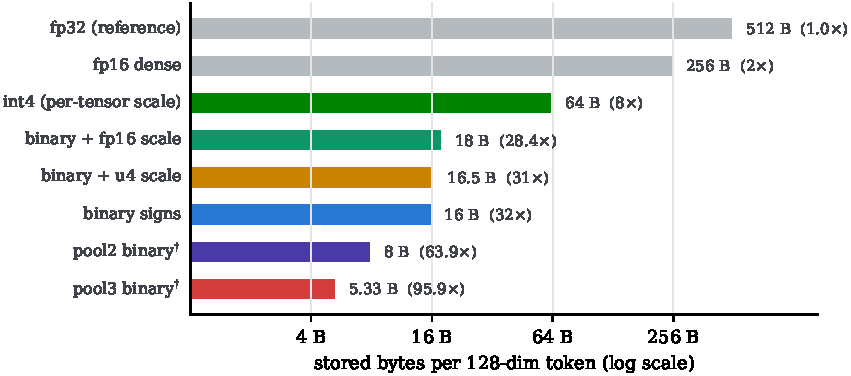
\includegraphics[width=.84\linewidth]{figures/format_layout.pdf}
\caption{Storage per 128-dimensional document token. Pooled-binary storage is
shown per original token at pooling factor three.}
\label{fig:formats}
\end{figure}

Figure~\ref{fig:formats} summarizes the storage ladder. All compressed
formats are built post hoc from document embeddings; the encoder is unchanged.

\textbf{Binary.} Each document value is replaced by its sign and packed into
one bit. Queries remain floating point. At dimension 128 this uses 16 bytes
per token, $16\times$ smaller than fp16 and $32\times$ smaller than fp32.

\textbf{Scaled binary.} One 4-bit logarithmic magnitude value is stored per
token and applied before the reducer. This restores magnitude information at
little storage cost, but it is only useful when that magnitude correlates
with retrieval salience.

\textbf{Pooled binary.} Document tokens are clustered independently within
each document, mean-pooled, and then binarized. Pool3 targets one stored vector
per three original vectors and reaches approximately $48\times$ compression
versus fp16, or $96\times$ versus fp32.

\textbf{Int4.} Two signed 4-bit values are packed per byte. We evaluate a
single tensor scale and one fp32 scale per token. The latter uses 68 bytes per
128-dimensional token and reaches $3.76\times$ compression versus fp16
($7.53\times$ versus fp32).

\textbf{Int8 control.} One int8 vector and one fp32 token scale use 132 bytes
per token. This format is less aggressive ($1.94\times$ versus fp16), but it
tests whether the model can be compressed with negligible quantization loss.

\textbf{Residual int4.} A second int4 stream represents the residual from the
first. Full scoring reconstructs both streams before reduction. It provides a
$1.88\times$ fp16 compression point intended for models that reject more
aggressive formats.

\subsection{CUDA runtime}

Packed document arrays and offsets remain GPU-resident. Binary paths unpack
signs inside the scoring kernel; int4 paths unpack nibbles and apply tensor or
token scales before reduction. Dim-128 fast paths use fixed-width vectorized
loads and measured launch policies. Candidate-only entry points gather only
the requested document ranges, which is important when \sysname{} is used as
a reranker behind an approximate or lexical first stage.

The current implementation uses specialized MaxSim entry points for its
long-established fast path and a shared reducer policy for the general
interface. The shared path was tuned on SM89, including removal of TopK4
register spills. Every reported kernel is checked against a PyTorch reference
with deterministic lower-index tie-breaking.

\section{Experimental Design}

\subsection{Quality matrix}

The primary matrix contains four encoder families. The text encoders are
Jina-ColBERT-v2~\citep{jha2024jina} and
GTE-ModernColBERT~\citep{chaffin2025pylate,chaffin2025gte}; the visual
encoders are ColPali-v1.3~\citep{faysse2025colpali} and the released
ColQwen2-v1.0 checkpoint~\citep{vidore2025colqwen2}.

\begin{center}
\small
\begin{tabular}{llll}
\toprule
encoder & modality & evaluation & datasets \\
\midrule
Jina-ColBERT-v2 & text & BEIR full test & FiQA, NFCorpus, SciFact \\
GTE-ModernColBERT & text & BEIR full test & FiQA, NFCorpus, SciFact \\
ColPali-v1.3 & visual & ViDoRe full test & 4 document QA sets \\
ColQwen2-v1.0 & visual & ViDoRe full test & 10 document QA sets \\
\bottomrule
\end{tabular}
\end{center}

The matrix contains 20 encoder--dataset cells. For Jina, GTE, and ColPali,
every format is evaluated on the same embeddings, query IDs, corpus, and
relevance judgments, with per-query \ndcg{} and \recall{} retained. ColQwen2
combines a historical dense/binary/pool sweep with later int4/int8 controls
joined by dataset metadata; because the historical files lack query
identifiers, per-query recall, and cache hashes, those cross-format deltas are
supporting rather than paired evidence.

For BEIR, all positive relevance labels are binarized to preserve
comparability with the historical GTE caches; the reported \ndcg{} therefore
uses binary relevance.

\subsection{End-to-end corpora and scale protocol}

The text end-to-end corpus is the full FiQA index encoded with
GTE-ModernColBERT: 57,638 documents and 648 queries. The visual corpus
contains 10,171 unique pages from public ViDoRe sources encoded with
ColQwen2; 2,000 selected queries are used. All formats report encoded bytes,
quality, latency, and throughput; compressed formats additionally report
serialized bytes and index construction/loading. These are production-path
benchmarks, not measurements of live serving traffic.

Nested-scale experiments use a fixed 256-query protocol and three corpus
seeds. Visual runs use 1k, 5k, and 10k documents; FiQA runs use 1k, 5k, 10k,
25k, and 57,638 documents. Every relevant document is retained as distractors
are added, so each method sees the same query set at every size within a seed.
There are 24 completed scale cases in total.

\subsection{Baselines and measurement}

Dense fp16 is vectorized as flat matrix multiplications over large
document-token chunks followed by segmented maxima. This avoids the severe
latency inflation of a Python document-by-document loop.
FastPLAID~\citep{santhanam2022plaid} is configured with 4-bit codes, four IVF
probes, and 4,096 full scores. It is an approximate index, whereas the
\sysname{} rows are full scans over their stored representations, so the
comparison is informative but not algorithmically identical.

All GPU measurements use one RTX~4090 (SM89). End-to-end latency uses three
warm-up calls and three measurements per query. Scale points use three timing
repeats. Small positive quality differences from dense in the visual
end-to-end table should not be read as improvements: the dense path stores
fp16 queries while some compressed paths receive fp32 queries, which can
change ties at the fourth decimal.

\section{Results}

\subsection{Compression is model-dependent}
\label{sec:quality}

\begin{figure}[t]
\centering
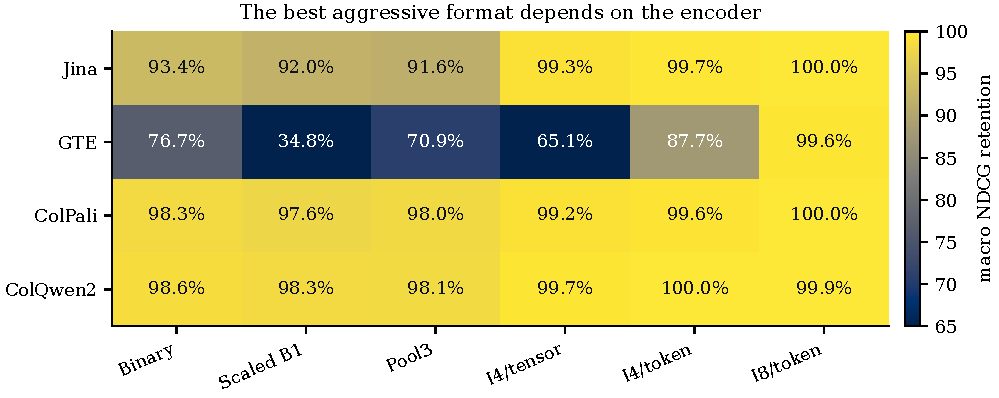
\includegraphics[width=.93\linewidth]{figures/model_format_heatmap.pdf}
\caption{Macro \ndcg{} retention relative to dense for four encoder families.
The same codec can be near-lossless for one encoder and unsafe for another.}
\label{fig:heatmap}
\end{figure}

\begin{table}[t]
\centering
\caption{Macro \ndcg{} across each model suite. Parenthesized values are
retention relative to dense. Compression ratios are relative to fp32.}
\label{tab:model-matrix}
\footnotesize
\resizebox{\linewidth}{!}{\begin{tabular}{lrrrrrrr}
\toprule
model & dense & binary & scaled B1 & pool3 & I4/tensor & I4/token & I8/token \\
\midrule
Jina & 0.4884 & 0.4560 (93.4\%) & 0.4492 (92.0\%) & 0.4475 (91.6\%) & 0.4850 (99.3\%) & 0.4871 (99.7\%) & 0.4882 (100.0\%) \\
GTE & 0.5310 & 0.4074 (76.7\%) & 0.1846 (34.8\%) & 0.3767 (70.9\%) & 0.3457 (65.1\%) & 0.4660 (87.7\%) & 0.5289 (99.6\%) \\
ColPali & 0.7856 & 0.7725 (98.3\%) & 0.7664 (97.6\%) & 0.7699 (98.0\%) & 0.7797 (99.2\%) & 0.7823 (99.6\%) & 0.7857 (100.0\%) \\
ColQwen2 & 0.4559 & 0.4497 (98.6\%) & 0.4482 (98.3\%) & 0.4473 (98.1\%) & 0.4544 (99.7\%) & 0.4557 (100.0\%) & 0.4554 (99.9\%) \\
\bottomrule
\end{tabular}
}
\end{table}

Figure~\ref{fig:heatmap} and Table~\ref{tab:model-matrix} contain the paper's
main finding. The formats fall into three qualitatively different groups.

\textbf{Per-token int8 is a robust control.} It retains 99.60--100.01\% of
macro dense \ndcg{} across the four model suites. Across the 10 directly
paired Jina, GTE, and ColPali cells, it stays within 0.0043 \ndcg{} of dense;
the largest joined ColQwen2 cell gap is 0.0063. This indicates that all four
embedding families tolerate a meaningful reduction in precision. The
trade-off is storage: int8 plus a token scale is only $3.88\times$ smaller
than fp32, and the release does not yet include a dedicated int8 CUDA latency
path.

\textbf{Per-token int4 is strong, but not universal.} It retains 99.75\% for
Jina, 99.58\% for ColPali, and 99.96\% for ColQwen2 at $7.53\times$
compression versus fp32. On GTE, however, retention falls to 87.75\% and the
macro deficit is 0.0651. A modality-only rule would miss this: both Jina and
GTE are text late-interaction encoders, yet they require different formats.
Tensor-scale int4 is less reliable still, retaining only 65.1\% on GTE.

\textbf{Binary and pooling are compelling on visual encoders.} Binary retains
98.33\% on ColPali and 98.65\% on ColQwen2 at $32\times$ compression. Pool3
retains 98.00\% and 98.11\% at approximately $96\times$. These averages hide
dataset variation: DocVQA is the most compression-sensitive ColPali dataset,
where pool3 loses 0.0319 \ndcg{}. The same modes are much weaker for GTE
(76.72\% and 70.94\% macro retention).

\textbf{Magnitude restoration is not automatically helpful.} Scaled binary
is close to binary for the visual encoders and Jina, but collapses on GTE:
FiQA falls from 0.4555 dense to 0.0710. The scale value's benefit is
encoder-dependent, so token magnitude cannot be treated as generic side
information.

The practical conclusion is stronger than selecting a new fixed default.
Compression should be calibrated \emph{per encoder}. A conservative int8
control determines whether quantization is viable, after which int4, binary,
and pooled-binary modes can be evaluated against an explicit quality budget.

\subsection{End-to-end deployment frontier}
\label{sec:production}

\begin{figure}[t]
\centering
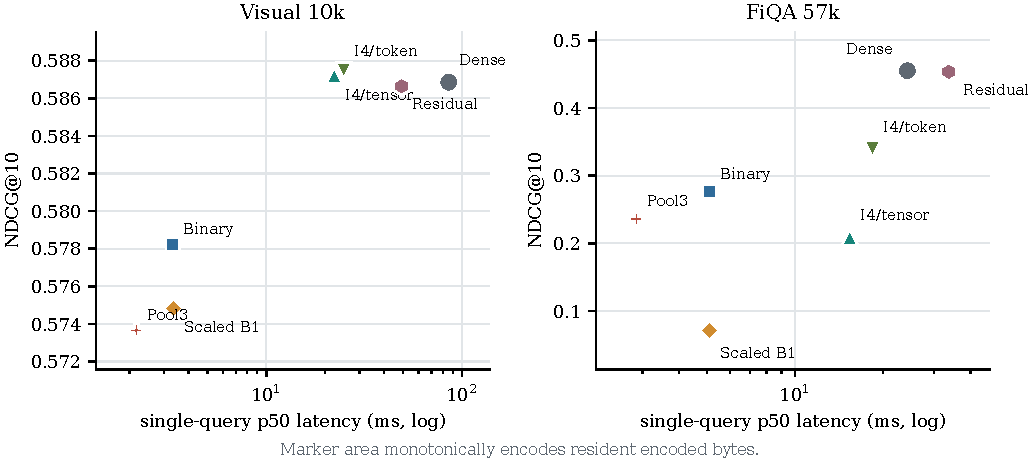
\includegraphics[width=.97\linewidth]{figures/production_frontier.pdf}
\caption{End-to-end quality, storage, and single-query latency on the visual
10k and FiQA 57k corpora. Points closer to the upper-left are preferable.}
\label{fig:production}
\end{figure}

\begin{table}[t]
\centering
\caption{End-to-end benchmark results on one RTX~4090. Speedup and
compression are relative to dense fp16 within each corpus.}
\label{tab:production}
\footnotesize
\resizebox{\linewidth}{!}{\begin{tabular}{llrrrrrrr}
\toprule
corpus & format & \ndcg{} & p50 ms & p95 ms & QPS & MiB & speedup & compr. \\
\midrule
Visual 10k & Dense & 0.5869 & 85.73 & 122.55 & 14.1 & 1852.6 & 1.00$\times$ & 1.0$\times$ \\
Visual 10k & Binary & 0.5782 & 3.32 & 4.90 & 329.0 & 115.8 & 25.80$\times$ & 16.0$\times$ \\
Visual 10k & Scaled B1 & 0.5748 & 3.36 & 4.96 & 334.4 & 119.4 & 25.53$\times$ & 15.5$\times$ \\
Visual 10k & Pool3 & 0.5736 & 2.17 & 3.16 & 522.1 & 38.6 & 39.56$\times$ & 47.9$\times$ \\
Visual 10k & I4/tensor & 0.5872 & 22.26 & 33.28 & 47.5 & 463.1 & 3.85$\times$ & 4.0$\times$ \\
Visual 10k & I4/token & 0.5875 & 24.85 & 35.97 & 46.7 & 492.1 & 3.45$\times$ & 3.8$\times$ \\
Visual 10k & Residual & 0.5866 & 49.26 & 70.98 & 23.5 & 984.2 & 1.74$\times$ & 1.9$\times$ \\
FiQA 57k & Dense & 0.4551 & 24.31 & 32.46 & 50.2 & 1878.7 & 1.00$\times$ & 1.0$\times$ \\
FiQA 57k & Binary & 0.2769 & 5.11 & 7.77 & 169.8 & 117.4 & 4.76$\times$ & 16.0$\times$ \\
FiQA 57k & Scaled B1 & 0.0710 & 5.10 & 7.77 & 170.2 & 121.1 & 4.76$\times$ & 15.5$\times$ \\
FiQA 57k & Pool3 & 0.2359 & 2.86 & 4.13 & 357.4 & 39.4 & 8.50$\times$ & 47.6$\times$ \\
FiQA 57k & I4/tensor & 0.2091 & 15.44 & 24.45 & 52.5 & 469.7 & 1.57$\times$ & 4.0$\times$ \\
FiQA 57k & I4/token & 0.3391 & 18.48 & 27.22 & 51.6 & 499.0 & 1.32$\times$ & 3.8$\times$ \\
FiQA 57k & Residual & 0.4536 & 33.72 & 50.87 & 27.0 & 998.1 & 0.72$\times$ & 1.9$\times$ \\
\bottomrule
\end{tabular}
}
\end{table}

The visual corpus exposes a wide useful frontier. Dense fp16 reaches 0.5869
\ndcg{} at 85.7\,ms p50 and 1.94\,GB. Binary reaches 0.5782 at 3.32\,ms using
121\,MB: $25.8\times$ lower latency and $16.0\times$ less storage. Pool3
reaches 0.5736 at 2.17\,ms and 40.5\,MB: $39.6\times$ lower latency and
$47.9\times$ less storage. Tensor and token int4 remain at dense quality
(within the precision caveat above) with p50 latencies of 22.3 and 24.8\,ms.
The result gives applications multiple meaningful operating points rather
than one fragile optimum.

FiQA with GTE is intentionally harder. Dense reaches 0.4551 at 24.3\,ms.
Binary and pool3 are fast (5.11 and 2.86\,ms) but retain only 60.8\% and
51.8\% of dense quality. Token int4 improves to 0.3391, but is not a
quality-preserving default. Residual int4 recovers 99.66\% of dense quality
at $1.88\times$ fp16 compression, though its 33.7\,ms p50 is slower than
dense. Compression remains useful here, but the relevant objective is
footprint rather than speed.

These two corpora demonstrate why a portfolio matters. On ColQwen2, binary
and pooling unlock both memory and latency; on GTE, a high-fidelity residual
format is the only latency-benchmarked compressed tier near dense quality.
Token int8 is near dense in the quality matrix but has no dedicated latency
path.

\subsection{Scaling is consistent, not universal}
\label{sec:scale}

\begin{figure}[t]
\centering
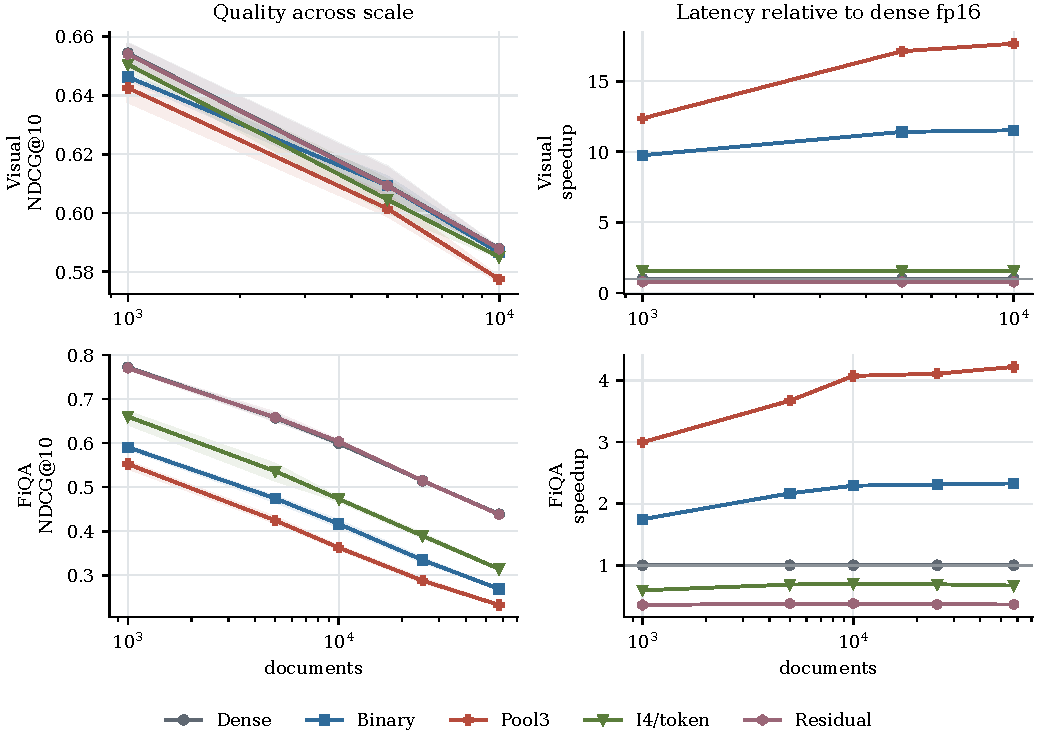
\includegraphics[width=.97\linewidth]{figures/scale_consistency.pdf}
\caption{Nested scale results over three corpus seeds. Lines show means and
bands show the seed range for the fixed 256-query protocol.}
\label{fig:scale}
\end{figure}

The controlled scale sweep replaces an earlier, query-set-dependent
observation that pooling overtook binary at large visual corpus sizes.
Figure~\ref{fig:scale} shows the reproducible result. On visual data, binary
and pool3 remain close to dense as the corpus grows, but binary consistently
has higher quality: at 10k documents dense, binary, and pool3 reach
0.5879, 0.5865, and 0.5774 mean \ndcg{}. Their speedups increase to
$11.5\times$ and $17.7\times$ for the 256-query workload.

On FiQA, speed also scales predictably: at 57,638 documents binary and pool3
are $2.33\times$ and $4.22\times$ faster than dense in the batched protocol.
Their quality deficits persist, and the scaled-binary failure remains severe.
Residual int4 follows dense quality closely at every size but is slower.

The system behavior is therefore stable enough to plan capacity, while the
quality behavior remains model-specific. Corpus size does not rescue a codec
that is poorly matched to the encoder.

\subsection{One runtime supports five reducers}
\label{sec:reducers}

\begin{figure}[t]
\centering
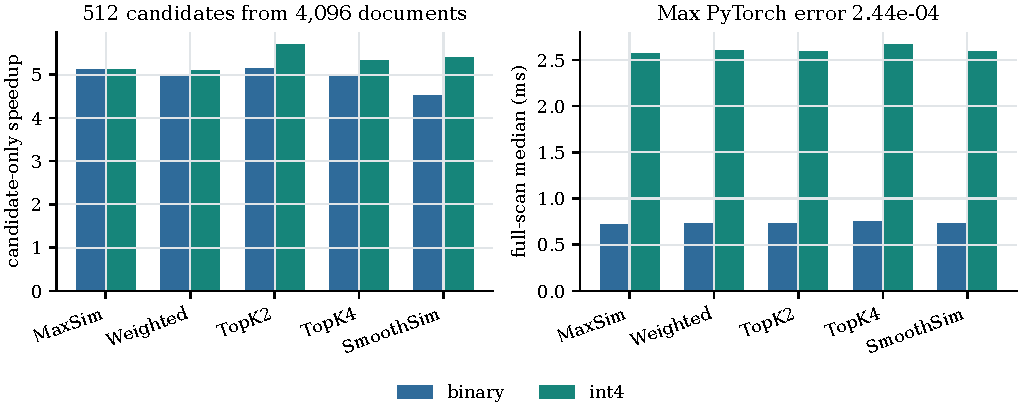
\includegraphics[width=.90\linewidth]{figures/reducer_generality.pdf}
\caption{Shared-reducer latency and candidate-only speedup at 4,096 documents.
All five reducers pass the PyTorch parity gate for binary and int4.}
\label{fig:reducers}
\end{figure}

The shared path covers MaxSim, weighted MaxSim, TopK2, TopK4, and SmoothSim.
At 4,096 documents and 512 candidates, candidate-only scoring is
$4.53\times$--$5.14\times$ faster than full scoring for binary and
$5.08\times$--$5.69\times$ for int4. At 512 documents, where launch overhead
is a larger fraction, the corresponding ranges are $1.30\times$--$1.53\times$
and $2.09\times$--$2.30\times$.

The shared MaxSim implementation is also faster than the legacy path at 4,096
documents: $1.12\times$ for binary and $1.04\times$ for int4. At 512
documents the binary gain is larger ($1.29\times$), while shared int4 is
effectively at parity ($1.01\times$). Across shared-reducer rows, maximum
deviation from PyTorch is $2.44{\times}10^{-4}$; including legacy comparison
rows, the maximum is $3.67{\times}10^{-4}$. This result supports a general
runtime claim for dot-product reducers without pretending that MaxSim
retrieval experiments establish the task quality of every reducer.

\subsection{Relation to PLAID}
\label{sec:plaid}

\begin{table}[t]
\centering
\caption{Matched FastPLAID measurements. PLAID is approximate; \sysname{}
rows are full scans over compressed representations, so index size and
latency are not strictly apples-to-apples.}
\label{tab:plaid}
\footnotesize
\resizebox{\linewidth}{!}{\begin{tabular}{llrrrr}
\toprule
corpus & system & \ndcg{} & \recall{} & p50 ms & index GB \\
\midrule
Visual 10k & FastPLAID & 0.5871 & 0.6445 & 15.79 & 1.126 \\
Visual 10k & \sysname{} Dense & 0.5869 & 0.6465 & 85.73 & 1.943 \\
Visual 10k & \sysname{} Binary & 0.5782 & 0.6440 & 3.32 & 0.121 \\
Visual 10k & \sysname{} Pool3 & 0.5736 & 0.6395 & 2.17 & 0.041 \\
Visual 10k & \sysname{} I4/tensor & 0.5872 & 0.6505 & 22.26 & 0.486 \\
Visual 10k & \sysname{} I4/token & 0.5875 & 0.6470 & 24.85 & 0.516 \\
Visual 10k & \sysname{} Residual & 0.5866 & 0.6465 & 49.26 & 1.032 \\
FiQA 57k & FastPLAID & 0.4524 & 0.5200 & 3.76 & 1.166 \\
FiQA 57k & \sysname{} Dense & 0.4551 & 0.5214 & 24.31 & 1.970 \\
FiQA 57k & \sysname{} Binary & 0.2769 & 0.3351 & 5.11 & 0.123 \\
FiQA 57k & \sysname{} Pool3 & 0.2359 & 0.2758 & 2.86 & 0.041 \\
FiQA 57k & \sysname{} I4/tensor & 0.2091 & 0.2752 & 15.44 & 0.492 \\
FiQA 57k & \sysname{} I4/token & 0.3391 & 0.3885 & 18.48 & 0.523 \\
FiQA 57k & \sysname{} Residual & 0.4536 & 0.5192 & 33.72 & 1.047 \\
\bottomrule
\end{tabular}
}
\end{table}

FastPLAID reaches near-dense quality on both corpora: 0.5871 \ndcg{} at
15.79\,ms p50 on visual 10k, and 0.4524 at 3.76\,ms on FiQA 57k. Its indexes
occupy 1.126 and 1.166\,GB. On visual data, \sysname{} tensor/token int4
provide comparable quality in roughly 0.49--0.52\,GB, while binary and pool3
trade a small quality loss for much lower latency and footprint. Pool3 is
approximately $27.8\times$ smaller than the PLAID index.

On FiQA, FastPLAID provides the best measured high-quality latency/quality
operating point: aggressive \sysname{} modes lose too much quality, and
residual int4 is slower. This is not a contradiction. PLAID prunes the corpus
using a learned index structure; \sysname{} is a model-agnostic compression
and scoring primitive. It can serve as a transparent full-scan index at
moderate scale or as the candidate reranker behind PLAID, BM25, or another
first stage.

\subsection{A practical selection policy}

\begin{table}[t]
\centering
\caption{Recommended deployment policy. ``Validate'' means evaluating the
mode on held-out queries from the target encoder and corpus.}
\label{tab:policy}
\small
\begin{tabular}{p{.20\linewidth}p{.25\linewidth}p{.47\linewidth}}
\toprule
goal & first mode & decision rule \\
\midrule
Near-lossless & token int8 & Use as the near-lossless control;
fall back to fp16 if the quality budget is unusually tight. \\
Quality and footprint & token int4 & Keep if validated; for visual encoders,
also test tensor int4. On FiQA/GTE, residual int4 was near dense; validate it
independently on other GTE corpora. \\
Lowest latency & binary & Keep only if the measured quality loss is
acceptable. Visual encoders are the strongest observed case. \\
Smallest index & pool3 binary & Validate per dataset; do not infer safety
from modality or corpus size. \\
\bottomrule
\end{tabular}
\end{table}

This policy is deliberately small. It does not require a search over every
quantizer parameter. Token int8 establishes a safe reference, and three
aggressive candidates cover the main quality--storage--latency regimes. The
library exposes the production formats through one API, so calibration
changes index construction rather than the surrounding retrieval system.
Token int8 is currently an offline calibration control without a dedicated
runtime path. The SDK's current \texttt{auto} alias resolves to token int4 and
should be treated as a convenience candidate, not as the model-aware selector
proposed here.

\section{Related Work}

\textbf{Late interaction.} ColBERT introduced token-level MaxSim for text
retrieval~\citep{khattab2020colbert}; ColBERTv2 combined late interaction with
residual compression~\citep{santhanam2022colbertv2}. PLAID accelerates
retrieval through centroid-based pruning~\citep{santhanam2022plaid}. ColPali
extends late interaction to visual document retrieval by embedding page
patches directly~\citep{faysse2025colpali}. \sysname{} is complementary: it
compresses already-produced document vectors and provides exact reductions
over the stored compressed representation.

\textbf{Quantization.} Scalar and integer quantization reduce model and vector
storage by mapping floating-point values to small discrete alphabets
\citep{jacob2018quant}. Product quantization compresses vectors using learned
subspace codebooks~\citep{jegou2011pq}; binary hashing and rotations such as
ITQ target compact similarity search~\citep{gong2013itq}. Our focus is
asymmetric dot-product late interaction, where the maximum over document
tokens makes errors and scale choices interact with ranking.

\textbf{Token reduction.} Token pruning and clustering reduce the number of
vectors stored per document. Prior work has shown that pooling can reduce the
multi-vector footprint with limited average impact
\citep{clavie2024pooling}. Recent visual-document work studies patch pruning
and merging for ColPali/ColQwen2 and develops
Light-ColPali/ColQwen2~\citep{ma2025storage}. Our work instead evaluates
post-hoc bit-level compression jointly with pooling and a CUDA scoring
runtime.

\textbf{Evaluation.} BEIR provides heterogeneous text retrieval tasks
\citep{thakur2021beir}; ViDoRe is used through the ColPali evaluation stack
\citep{faysse2025colpali}. Our contribution is not a new embedding model or
benchmark, but a controlled map of compression behavior across existing
families and deployment shapes.

\section{Limitations}

The study covers four encoder families, text and visual retrieval, and
corpora up to 57,638 documents. This is enough to show that none of the
evaluated aggressive formats is universally safe across the tested encoders,
but not enough to prove the selection policy optimal for all future encoders
or million-document deployments.

All evaluated encoders emit 128-dimensional vectors. The API supports fixed
dimensions divisible by eight, but the performance claims in this paper are
for dimension 128.

End-to-end retrieval quality is measured with MaxSim. The five-reducer result
establishes numerical correctness and runtime generality for dot-product
late-interaction scorers; it does not establish task quality for weighted,
top-$k$, or smooth reducers. Per-token int8 is a quality control without a
dedicated CUDA latency kernel in this release. A label-aware automatic
selector is not yet implemented; deployment currently uses explicit modes.

All latency data comes from one RTX~4090. Absolute performance and kernel
ordering may change on other architectures. The dense and compressed visual
end-to-end paths differ slightly in query precision, so fourth-decimal gains
over dense are treated as ties.

FastPLAID and \sysname{} implement different search algorithms. PLAID uses
approximate pruning and a learned index; \sysname{} reports exact full scans
over a compressed representation. We report both because practitioners need
the comparison, but do not present their latency as a controlled kernel
ablation.

The paper bundle contains the complete new model and systems runs, including
result JSONs, logs, checksums, and source-cache hashes. Historical ColQwen2
dense/binary/pool rows remain in the repository ledger and are treated as
supporting evidence. Eight newly generated raw embedding caches were excluded
because of size, so reproducing those runs requires re-encoding.

\section*{Reproducibility Statement}

The authoritative bundle is
\path{benchmark-results/paper-20260715}. Its SHA-256 manifest covers the
archived model and systems results. Model-quality runs identify source commit
\texttt{88fff9e}. The archive README identifies systems source
\texttt{e213917e}; the systems environment field contains the malformed hash
documented in the Appendix. Every generated table and figure in this
manuscript is produced by \texttt{paper/make\_paper\_artifacts.py}, which
validates completion status, required result fields, expected dataset counts,
and the explicit ColQwen2 legacy/new join before writing paper artifacts.

End-to-end JSONs retain raw per-query timing samples, rankings, quality
vectors, storage reports, and run signatures. Scale runs retain all three
seeds at every size. Reducer artifacts retain the exact shapes, implementations,
latencies, and PyTorch errors. The archived experiment workers each report 80
passing CUDA-selected tests. The release-validation artifact records 80 CUDA
tests, 223 non-CUDA tests, and zero errors across Compute Sanitizer memcheck,
initcheck, racecheck, and synccheck.

\section{Conclusion}

Multi-vector retrieval does not need a single universal codec to become
practical. It needs a small, well-measured portfolio. Across four encoder
families, per-token int8 is consistently near dense, per-token int4 is an
excellent aggressive format for Jina and visual encoders, binary and pooling
produce large visual speedups, and GTE requires higher fidelity. The same
runtime supports five reducers and efficient candidate reranking.

The resulting default is a procedure, not a constant: establish a
near-lossless control, validate a few aggressive modes on the target encoder,
and choose the smallest representation that satisfies the application's
quality budget. \sysname{} supports deploying the selected production format
through one index API, with parity-tested CUDA kernels and reproducible
evidence.

\begin{thebibliography}{15}

\bibitem[Khattab and Zaharia(2020)]{khattab2020colbert}
O.~Khattab and M.~Zaharia.
\newblock ColBERT: Efficient and effective passage search via contextualized
late interaction over BERT.
\newblock In \emph{SIGIR}, 2020.

\bibitem[Santhanam et~al.(2022a)]{santhanam2022colbertv2}
K.~Santhanam, O.~Khattab, J.~Saad-Falcon, C.~Potts, and M.~Zaharia.
\newblock ColBERTv2: Effective and efficient retrieval via lightweight late
interaction.
\newblock In \emph{NAACL}, 2022.

\bibitem[Santhanam et~al.(2022b)]{santhanam2022plaid}
K.~Santhanam, O.~Khattab, C.~Potts, and M.~Zaharia.
\newblock PLAID: An efficient engine for late interaction retrieval.
\newblock In \emph{CIKM}, 2022.

\bibitem[Faysse et~al.(2025)]{faysse2025colpali}
M.~Faysse, H.~Sibille, T.~Wu, B.~Omrani, G.~Viaud, C.~Hudelot, and P.~Colombo.
\newblock ColPali: Efficient document retrieval with vision language models.
\newblock In \emph{International Conference on Learning Representations},
2025.

\bibitem[Jha et~al.(2024)]{jha2024jina}
R.~Jha, B.~Wang, M.~G\"unther, G.~Mastrapas, S.~Sturua, I.~Mohr,
A.~Koukounas, M.~K. Akram, N.~Wang, and H.~Xiao.
\newblock Jina-ColBERT-v2: A general-purpose multilingual late interaction
retriever.
\newblock In \emph{MRL}, pages 159--166, 2024.

\bibitem[Chaffin and Sourty(2025)]{chaffin2025pylate}
A.~Chaffin and R.~Sourty.
\newblock PyLate: Flexible training and retrieval for late interaction
models.
\newblock In \emph{CIKM}, pages 6334--6339, 2025.

\bibitem[Chaffin(2025)]{chaffin2025gte}
A.~Chaffin.
\newblock GTE-ModernColBERT-v1 model card.
\newblock \url{https://huggingface.co/lightonai/GTE-ModernColBERT-v1}, 2025.

\bibitem[ViDoRe(2025)]{vidore2025colqwen2}
ViDoRe.
\newblock ColQwen2-v1.0-HF model repository, revision
\texttt{b8a106812c8682bab08935cf5d1b4566c82562de}.
\newblock \url{https://huggingface.co/vidore/colqwen2-v1.0-hf}, 2025.

\bibitem[Thakur et~al.(2021)]{thakur2021beir}
N.~Thakur, N.~Reimers, A.~R\"uckl\'e, A.~Srivastava, and I.~Gurevych.
\newblock BEIR: A heterogeneous benchmark for zero-shot evaluation of
information retrieval models.
\newblock In \emph{NeurIPS Datasets and Benchmarks}, 2021.

\bibitem[J{\'e}gou et~al.(2011)]{jegou2011pq}
H.~J{\'e}gou, M.~Douze, and C.~Schmid.
\newblock Product quantization for nearest neighbor search.
\newblock \emph{IEEE TPAMI}, 33(1), 2011.

\bibitem[Gong et~al.(2013)]{gong2013itq}
Y.~Gong, S.~Lazebnik, A.~Gordo, and F.~Perronnin.
\newblock Iterative quantization: A Procrustean approach to learning binary
codes for large-scale image retrieval.
\newblock \emph{IEEE TPAMI}, 35(12), 2013.

\bibitem[Jacob et~al.(2018)]{jacob2018quant}
B.~Jacob, S.~Kligys, B.~Chen, M.~Zhu, M.~Tang, A.~Howard, H.~Adam, and
D.~Kalenichenko.
\newblock Quantization and training of neural networks for efficient
integer-arithmetic-only inference.
\newblock In \emph{CVPR}, 2018.

\bibitem[Clavi{\'e} et~al.(2024)]{clavie2024pooling}
B.~Clavi{\'e}, A.~Chaffin, and G.~Adams.
\newblock Reducing the footprint of multi-vector retrieval with minimal
performance impact via token pooling.
\newblock \emph{arXiv:2409.14683}, 2024.

\bibitem[Ma et~al.(2025)]{ma2025storage}
Y.~Ma, J.~Li, Y.~Zang, X.~Wu, X.~Dong, P.~Zhang, Y.~Cao, H.~Duan,
J.~Wang, Y.~Cao, and A.~Sun.
\newblock Towards storage-efficient visual document retrieval: An empirical
study on reducing patch-level embeddings.
\newblock In \emph{Findings of ACL}, pages 19568--19580, 2025.

\end{thebibliography}

\clearpage
\appendix

\section{Exact Per-Dataset Quality}
\label{app:quality}

\begin{center}
\captionof{table}{Text \ndcg{} by dataset for Jina-ColBERT-v2 and
GTE-ModernColBERT.}
\label{tab:text-exact}
\footnotesize
\resizebox{\linewidth}{!}{\begin{tabular}{lrrrrrrr}
\toprule
model / dataset & dense & binary & scaled B1 & pool3 & I4/tensor & I4/token & I8/token \\
\midrule
Jina / FiQA & 0.4151 & 0.3800 & 0.3618 & 0.3553 & 0.4069 & 0.4138 & 0.4147 \\
Jina / NFCorpus & 0.3564 & 0.3213 & 0.3216 & 0.3282 & 0.3536 & 0.3551 & 0.3566 \\
Jina / SciFact & 0.6935 & 0.6667 & 0.6642 & 0.6591 & 0.6945 & 0.6925 & 0.6933 \\
GTE / FiQA & 0.4555 & 0.2769 & 0.0710 & 0.2359 & 0.2091 & 0.3391 & 0.4538 \\
GTE / NFCorpus & 0.3768 & 0.2670 & 0.1558 & 0.2430 & 0.3233 & 0.3608 & 0.3764 \\
GTE / SciFact & 0.7608 & 0.6783 & 0.3269 & 0.6513 & 0.5047 & 0.6980 & 0.7565 \\
\bottomrule
\end{tabular}
}
\end{center}

\begin{center}
\captionof{table}{Visual \ndcg{} by dataset for ColPali-v1.3 and ColQwen2-v1.0.
ColQwen2 controls joined from the later run are marked in the generated
table.}
\label{tab:visual-exact}
\footnotesize
\resizebox{\linewidth}{!}{\begin{tabular}{lrrrrrrr}
\toprule
model / dataset & dense & binary & scaled B1 & pool3 & I4/tensor & I4/token & I8/token \\
\midrule
ColPali / ArxivQA & 0.8429 & 0.8278 & 0.8275 & 0.8309 & 0.8398 & 0.8410 & 0.8430 \\
ColPali / DocVQA & 0.5563 & 0.5390 & 0.5148 & 0.5244 & 0.5369 & 0.5451 & 0.5565 \\
ColPali / InfoVQA & 0.8579 & 0.8433 & 0.8438 & 0.8416 & 0.8550 & 0.8573 & 0.8578 \\
ColPali / TabFQuAD & 0.8854 & 0.8799 & 0.8794 & 0.8826 & 0.8871 & 0.8860 & 0.8854 \\
ColQwen2$^\dagger$ / ArxivQA & 0.8786 & 0.8623 & 0.8591 & 0.8565 & 0.8685 & 0.8721 & 0.8723 \\
ColQwen2$^\dagger$ / DocVQA & 0.5747 & 0.5546 & 0.5505 & 0.5576 & 0.5678 & 0.5724 & 0.5728 \\
ColQwen2$^\dagger$ / InfoVQA & 0.9088 & 0.8977 & 0.8979 & 0.8950 & 0.9085 & 0.9086 & 0.9098 \\
ColQwen2$^\dagger$ / TabFQuAD & 0.8865 & 0.8858 & 0.8834 & 0.8860 & 0.8919 & 0.8904 & 0.8878 \\
ColQwen2$^\dagger$ / TAT-DQA & 0.8120 & 0.8022 & 0.7977 & 0.7876 & 0.8081 & 0.8132 & 0.8114 \\
ColQwen2$^\dagger$ / Synth/AI & 0.1035 & 0.1024 & 0.1028 & 0.1022 & 0.1031 & 0.1035 & 0.1035 \\
ColQwen2$^\dagger$ / Synth/Energy & 0.1011 & 0.1004 & 0.1001 & 0.0996 & 0.1012 & 0.1011 & 0.1017 \\
ColQwen2$^\dagger$ / Synth/Gov. & 0.1012 & 0.1012 & 0.1008 & 0.0991 & 0.1018 & 0.1021 & 0.1017 \\
ColQwen2$^\dagger$ / Synth/Health & 0.1013 & 0.1024 & 0.1018 & 0.1019 & 0.1011 & 0.1016 & 0.1018 \\
ColQwen2$^\dagger$ / Synth/Shift & 0.0912 & 0.0883 & 0.0879 & 0.0874 & 0.0926 & 0.0920 & 0.0916 \\
\bottomrule
\end{tabular}
}
\end{center}

\section{Scale and Reducer Details}

\begin{center}
\captionof{table}{Mean nested-scale results across three seeds. Latency speedup is
relative to dense fp16 at the same corpus size.}
\label{tab:scale-exact}
\footnotesize
\resizebox{\linewidth}{!}{\begin{tabular}{lrrrrrr}
\toprule
corpus & docs & dense & binary & B1 speed & pool3 & P3 speed \\
\midrule
Visual & 1,000 & 0.6544 & 0.6463 & 9.75$\times$ & 0.6426 & 12.36$\times$ \\
Visual & 5,000 & 0.6094 & 0.6093 & 11.41$\times$ & 0.6015 & 17.12$\times$ \\
Visual & 10,000 & 0.5879 & 0.5865 & 11.52$\times$ & 0.5774 & 17.66$\times$ \\
FiQA & 1,000 & 0.7724 & 0.5907 & 1.75$\times$ & 0.5525 & 3.00$\times$ \\
FiQA & 5,000 & 0.6573 & 0.4743 & 2.17$\times$ & 0.4244 & 3.67$\times$ \\
FiQA & 10,000 & 0.5996 & 0.4164 & 2.29$\times$ & 0.3626 & 4.08$\times$ \\
FiQA & 25,000 & 0.5144 & 0.3342 & 2.31$\times$ & 0.2876 & 4.11$\times$ \\
FiQA & 57,638 & 0.4387 & 0.2689 & 2.33$\times$ & 0.2323 & 4.22$\times$ \\
\bottomrule
\end{tabular}
}
\end{center}

\begin{center}
\captionof{table}{Shared-reducer parity and latency at 512 and 4,096 documents.}
\label{tab:reducers-exact}
\footnotesize
\resizebox{\linewidth}{!}{\begin{tabular}{rrlrrrr}
\toprule
docs & format & reducer & full ms & cand. ms & speedup & max error \\
\midrule
512 & binary & maxsim & 0.140 & 0.107 & 1.30$\times$ & 1.8e-04 \\
512 & binary & weighted\_maxsim & 0.146 & 0.105 & 1.40$\times$ & 2.4e-04 \\
512 & binary & topk2 & 0.132 & 0.094 & 1.40$\times$ & 1.8e-04 \\
512 & binary & topk4 & 0.140 & 0.091 & 1.53$\times$ & 1.2e-04 \\
512 & binary & smoothsim & 0.139 & 0.099 & 1.40$\times$ & 2.4e-04 \\
512 & int4 & maxsim & 0.455 & 0.203 & 2.24$\times$ & 2.4e-04 \\
512 & int4 & weighted\_maxsim & 0.471 & 0.222 & 2.13$\times$ & 2.4e-04 \\
512 & int4 & topk2 & 0.440 & 0.192 & 2.30$\times$ & 1.8e-04 \\
512 & int4 & topk4 & 0.469 & 0.225 & 2.09$\times$ & 1.8e-04 \\
512 & int4 & smoothsim & 0.470 & 0.207 & 2.27$\times$ & 1.8e-04 \\
4,096 & binary & maxsim & 0.724 & 0.142 & 5.11$\times$ & 2.4e-04 \\
4,096 & binary & weighted\_maxsim & 0.730 & 0.148 & 4.94$\times$ & 2.4e-04 \\
4,096 & binary & topk2 & 0.727 & 0.141 & 5.14$\times$ & 1.8e-04 \\
4,096 & binary & topk4 & 0.748 & 0.150 & 5.00$\times$ & 1.2e-04 \\
4,096 & binary & smoothsim & 0.729 & 0.161 & 4.53$\times$ & 2.4e-04 \\
4,096 & int4 & maxsim & 2.574 & 0.504 & 5.11$\times$ & 2.4e-04 \\
4,096 & int4 & weighted\_maxsim & 2.605 & 0.513 & 5.08$\times$ & 2.4e-04 \\
4,096 & int4 & topk2 & 2.586 & 0.455 & 5.69$\times$ & 2.4e-04 \\
4,096 & int4 & topk4 & 2.664 & 0.499 & 5.34$\times$ & 1.8e-04 \\
4,096 & int4 & smoothsim & 2.591 & 0.480 & 5.40$\times$ & 2.4e-04 \\
\bottomrule
\end{tabular}
}
\end{center}

\section{Cascade Decision}

Residual cascades were evaluated on FiQA with candidate budgets 100, 200, and
400. They recovered 94.6--99.4\% of the quality gap between the prefix and
full residual representation, but achieved only $1.01\times$--$1.02\times$
speedup relative to full residual scoring and added 78--81\% latency over the
prefix. Because the FiQA gate failed, the planned visual cascade replication
was skipped. Cascading is therefore implemented as an optional composition,
but it is not part of the paper's recommended core portfolio.

\end{document}
